\section{Il simulatore Alchemist}
Alchemist \cite{Pianini2013} è un simulatore stocastico nato come progetto all'interno dell'Università di Bologna, che permette la simulazione di scenari inerenti la computazione pervasiva, aggregata ed ispirata alla natura.
\newline
Alchemist si basa sull'algoritmo di simulazione stocastica (SSA) \textit{Next Reaction Method} \cite{Gibson2000} che è una versione più efficiente dell'algoritmo di Gillespie \cite{Gillespie1977}.

\subsection{Modello di dominio}
Le entità costituenti il meta-modello fondante di Alchemist, di cui viene fornita una rappresentazione grafica in figura \ref{fig:alchemist-model}, sono fortemente ispirate al mondo della chimica, come anche il nome del simulatore suggerisce:
\begin{itemize}
 \item \textbf{Molecola}: corrispettivo del concetto di variabile in un linguaggio di programmazione.
 \item \textbf{Concentrazione}: valore associato ad una particolare molecola.
 \item \textbf{Nodo}: contenitore di molecole e reazioni.
 \item \textbf{Ambiente}: esprime il concetto di spazio e contiene i nodi, gestendo la loro posizione e il loro movimento al suo interno.
 \item \textbf{Regola di collegamento}: funzione che associa ad ogni nodo un vicinato.
 \item \textbf{Vicinato}: insieme di nodi in relazione tra loro per mezzo di una regola di collegamento.
 \item \textbf{Reazione}: un qualsiasi evento che può cambiare lo stato dell'ambiente. È costituita da condizioni e azioni.
 \item \textbf{Distribuzione temporale}: funzione che esprime gli istanti temporali nei quali una reazione deve avvenire.
 \item \textbf{Condizione}: funzione che determina l'eventuale esecuzione e la frequenza delle azioni contenute in una reazione.
 \item \textbf{Azione}: cambiamento dell'ambiente che scaturisce da una reazione.
\end{itemize}
Nonostante questa natura apparentemente molto specifica, la principale caratteristica del simulatore è quella della generalità, che viene raggiunto attraverso l'uso delle \textbf{incarnazioni}, istanze concrete del meta-modello in cui ogni entità viene mappata ad un corrispettivo concetto dell'universo di interesse.
Le incarnazioni attualmente esistenti in Alchemist sono:
\begin{itemize}
 \item \textbf{Protelis}: incentrata sul linguaggio Protelis \cite{Pianini2015} e la programmazione aggregata, lo studio di dinamiche collettive a partire dall'interazione non coordinata delle singole entità.
 \item \textbf{SAPERE}: per la simulazione di scenari che traggono ispirazione da ecosistemi naturali.
 \item \textbf{Biochemistry}: utilizzata per sistemi cellulari, reazioni chimiche e più in generale per tutto il mondo della biochimica.
 \item \textbf{Scafi}: anch'essa dedicata alla programmazione aggregata ma basata sul framework scafi \cite{Casadei2016}.
\end{itemize}

\begin{figure}
  \centering
  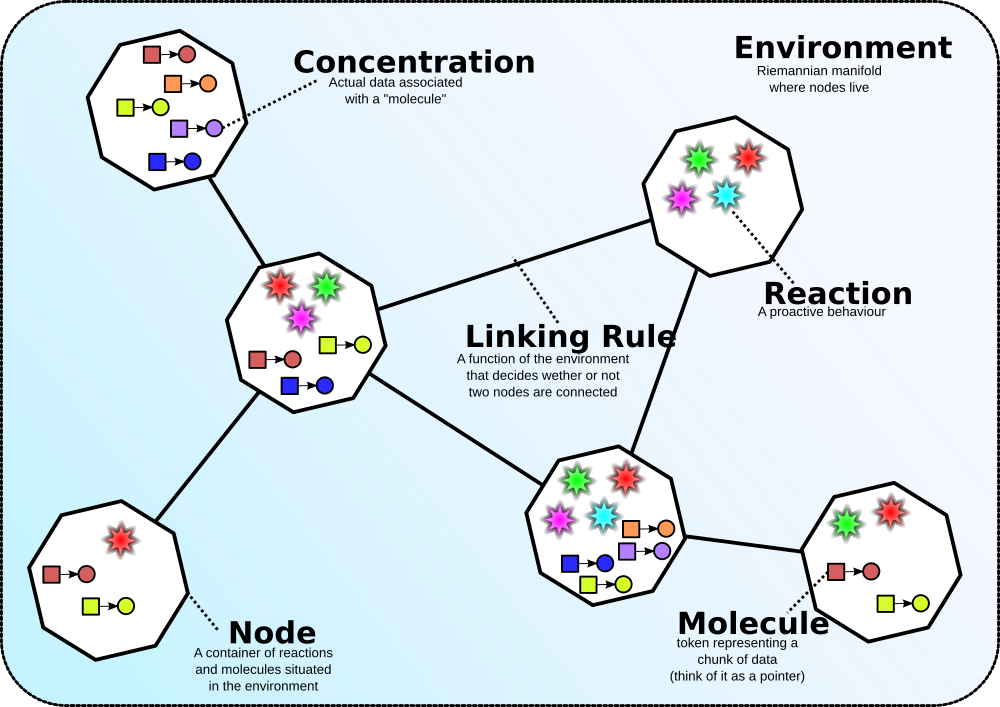
\includegraphics[width=0.80\linewidth]{immagini/alchemist-model.png}
  \caption{Il metamodello alla base di Alchemist.}
  \label{fig:alchemist-model}
\end{figure}

\subsection{Funzionalità}

\paragraph{Esecuzione batch} Al fine di poter effettuare dei confronti al variare dei parametri usati, Alchemist offre delle funzionalità batch, grazie alle quali una simulazione viene ripetuta per ogni valore nel range specificato.

\paragraph{Caricamento planimetrie} L'\texttt{ImageEnvironment} tra gli ambienti utilizzabili nelle simulazioni, permette il caricamento di una planimetria a partire da un'immagine, convertendo i pixel adiacenti del colore specificato in ostacoli.

\paragraph{Mappe geografiche} Il supporto agli standard GPX e GPS rende possibile il caricamento di mappe all'interno di  ambienti di tipo \texttt{MapEnvironment}, utili, ad esempio, in uno scenario di analisi del traffico stradale.

\paragraph{Calcolo distribuito} Considerata la possibilità di dover simulare scenari computazionalmente molto ardui da gestire, Alchemist offre il supporto ai sistemi grid, in cui il carico di lavoro viene suddiviso tra più calcolatori collegati alla medesima rete.

\subsection{Utilizzo}
Il linguaggio predefinito per la scrittura delle simulazioni in Alchemist è YAML\n{\url{https://yaml.org}}, uno standard di serializzazione dati facilmente leggibile anche dagli esseri umani. \newline
L'unico parametro da specificare obbligatoriamente per la corretta esecuzione di una simulazione è l'incarnazione da utilizzare, tutti gli altri parametri sono o indotti a partire da essa o specificati al fine di fornire ulteriori dettagli dello scenario di interesse. \newline
La principali chiavi utilizzabili all'interno di un file di simulazione Alchemist sono:
\begin{itemize}
    \item \texttt{incarnation}: l'incarnazione da utilizzare tra \texttt{protelis}, \texttt{sapere}, \texttt{biochemistry} e \texttt{scafi}.
    \item \texttt{seeds}: specifica i \textit{semi} da utilizzare per la generazione di numeri casuali. Ve ne sono solo due, \texttt{scenario} e \texttt{simulation}, impiegati rispettivamente per la creazione e l'esecuzione della simulazione.
    \item \texttt{variables}: valori che si vogliono riutilizzare all'interno del file di simulazione. Possono rappresentare sia semplici numeri che oggetti complessi come classi.
    \item \texttt{environment}: la tipologia di ambiente all'interno del quale si svolge la simulazione.
    \item \texttt{network-model}: la regola di collegamento con la quale sono associati i vari nodi.
    \item \texttt{displacements}: le posizioni in cui sono collocati i nodi all'inizio della simulazione.
    \item \texttt{layers}: gli strati rappresentanti le concentrazioni di determinate molecole in ogni punto dell'ambiente.
\end{itemize}
Per una descrizione più dettagliata delle chiavi utilizzabili si può far riferimento al sito ufficiale del simulatore\n{\url{https://alchemistsimulator.github.io/wiki/usage/yaml/}}.

\subsection{Accorgimenti}
Riuscire a riprodurre, a partire da una stessa configurazione di partenza codificata nel file YAML, delle simulazioni sempre identiche tra loro, è una prerogativa essenziale del simulatore Alchemist, senza la quale si andrebbe ad incorrere in problemi di irriproducibilità della stessa con conseguente non verificabilità dei risultati ottenuti. \newline
Al fine di ottemperare a questo punto cardine, nella scrittura di nuovi componenti da integrare all'interno di Alchemist, è necessario ricordare che non è possibile utilizzare un generatore di numeri pseudo-casuali diverso da quello di cui è provvista la simulazione. Inoltre, l'utilizzo di strutture dati quali \texttt{Set} o \texttt{Map} è consentito solo quando è possibile predeterminate l'ordine degli elementi al loro interno. \newline 
Ovviamente tali accorgimenti devono essere adottati anche nell'utilizzo di una libreria esterna, le cui classi non possono quindi essere usate come una \textit{scatola nera}.